\documentclass[a4paper,oneside,12pt]{book}

%----------------------------------------------------------------------------------------
%	README!
%   Welcome. It's worth having a read through this file
%   to set up the broad parameters, such as the name of
%   the degree, the school/department, the type of work
%   (dissertation/Final Year Project/report, etc. as well
%   as your own details.
%----------------------------------------------------------------------------------------

%----------------------------------------------------------------------------------------
%	COVER PAGE
%   The cover page is laid out in title/title.tex. You can choose a colour
%   or black and white logo
%----------------------------------------------------------------------------------------

%----------------------------------------------------------------------------------------
%	THESIS INFORMATION
%   Put title, author name, degree, type of work, school, department in here
%   It will be used for the title page and for the embedded PDF information
%----------------------------------------------------------------------------------------

\newcommand{\thesistitle}{Title of Work} % Your thesis title, this is used in the title and abstract
\newcommand{\degree}{B.A. (Mod.) Nanoscience, Physics \& Chemistry of Advanced Materials} % Your degree name, this is used in the title page and abstract
\newcommand{\typeofthesis}{Thesis} % dissertation, Final Year Project, report, etc.
\newcommand{\authorname}{Firstname Surname } % Your name, this is used in the title page and PDF stuff
%% Do not put your Student ID in the document, as TCD will not publish
%% documents that contain both your name and your Student ID.

\newcommand{\keywords}{this, that, more} % Keywords for your thesis
\newcommand{\school}{\href{https://chemistry.tcd.ie/}{School of Chemistry}} % Your school's name and URL, this is used in the title page

%% Comment out the next line if you don't want a department to appear
%\newcommand{\department}{\href{http://researchgroup.university.com}{Prof. Peter Dunne}} % Your research group's name and URL, this is used in the title page

\AtBeginDocument{
\hypersetup{pdftitle=\thesistitle} % Set the PDF's title to your title
\hypersetup{pdfauthor=\authorname} % Set the PDF's author to your name
\hypersetup{pdfkeywords=\keywords} % Set the PDF's keywords to your keywords
\hypersetup{pdfsubject=\degree} % Set the PDF's keywords to your keywords
}

%% Language and font encodings
\usepackage[T1]{fontenc} 
\usepackage[utf8]{inputenc}
\usepackage{lipsum}
\usepackage{ragged2e} %allows for text alignment preferences

%% Bibliographical stuff
\usepackage[round,sort,comma,numbers]{natbib}

%% Document size
% include showframe as an option if you want to see the boxes
\usepackage[a4paper,top=2.56cm,bottom=2.56cm,left=2.56cm,right=2.56cm, head = 16pt]{geometry}
\setlength{\marginparwidth}{2cm}
%% Useful packages
\usepackage{amsmath}
\usepackage[autostyle=true]{csquotes} % Required to generate language-dependent quotes in the bibliography
\usepackage[pdftex]{graphicx}
\usepackage[colorinlistoftodos]{todonotes}
\usepackage[colorlinks=true, allcolors=black]{hyperref}
\usepackage{xcolor}
\usepackage{caption} % if no caption, no colon
%\usepackage{sfmath} %use sans-serif in the maths sections too
\usepackage[parfill]{parskip}    % Begin paragraphs with an empty line rather than an indent
\usepackage{setspace} % to permit one-and-a-half or double spacing
\usepackage{enumerate} % fancy enumerations like (i) (ii) or (a) (b) and suchlike
\usepackage{booktabs} % To thicken table lines
\usepackage{fancyhdr}


%\pagestyle{plain} % Embrace simplicity!

%% The Mechanical engineers require your name and ID on the top of every page.
%% Uncomment the following block if you want your name and ID at the top of
%% (almost) every page.


\pagestyle{fancy}
\fancyhf{} % sets both header and footer to nothing
\renewcommand{\headrulewidth}{0pt}
\cfoot{\thepage}
%\ifdefined\authorid
%\chead{\it \authorname\ (\authorid)}
%\else
%\chead{\it \authorname}
%\fi
%% End of block

%% It is not a requirement of the university that the font should be sans-serif, but
%% the Mechanical engineers require it. Comment out the following line to disable it
%%\renewcommand{\familydefault}{\sfdefault} %use the sans-serif font as default

%% If you're not using sans-serif, consider using Palatino instead of the LaTeX standard
\usepackage{mathpazo} % Use the Palatino font by default if you prefer it to Computer Modern

\renewcommand{\theequation}{\arabic{equation}} %% use continuous equation numbers

%% Format Chapter headings appropriately
\usepackage{titlesec}
\usepackage{xepersian}


\definecolor{tcdblue}{cmyk}{0.94, 0.38, 0, 0.27}
\newcommand{\hsp}{\hspace{20pt}}
\titleformat{\chapter}[hang]{\Huge\bfseries}{\thechapter\hsp\textcolor{tcdblue}{|}\hsp}{0pt}{\Huge\bfseries}

\title{Logic design lab}
\author{Alireza Habibzadeh}

\frontmatter
\settextfont{FreeFarsi}

\begin{document}
\begin{titlepage}

\center % Center everything on the page

%% All the text parameters should be taken from the start of the main.tex file.
%% You should only alter stuff here if you want to change the layout

%----------------------------------------------------------------------------------------
%	LOGO SECTION
%----------------------------------------------------------------------------------------
%% Choose one of the following -- a colour or black-and-white logo


\includegraphics[width=0.3\textwidth]{title/logo.png}\\[1cm] 
%
\includegraphics[width=12cm]{title/black-stacked-trinity.jpg}\\[1cm] 
\ifdefined\school
\Large \textsc{گزارش‌کار اول آزمایشگاه مدارهای منطقی} \\[1.5cm] % Minor heading such as course title
\ifdefined\department
\large گزارش‌کار اول آزمایشگاه مدارهای منطقی\\[1.5cm] % Minor heading such as course title
\fi

%----------------------------------------------------------------------------------------
%	TITLE SECTION
%----------------------------------------------------------------------------------------
\makeatletter
\textsc{{ \huge \bfseries آشنایی با محیط‌های شبیه‌سازی}}\\[cm] % Title of your document
 

%----------------------------------------------------------------------------------------
%	AUTHOR SECTION
%----------------------------------------------------------------------------------------

\ifdefined\authorid
علیرضا حبیب‌زاده\\ % Your name
\authorid\\[2cm] % Your Student ID
\else
\textsc{
دکتر شاهین حسابی
}\\[2cm]
\fi

%----------------------------------------------------------------------------------------
%	DATE SECTION
%----------------------------------------------------------------------------------------

\textsc{{\large آبان 1400}}\\[2cm] % Date, change the \today to a set date if you want to be precise

\textcolor{black}{
نویسنده:
علیرضا حبیب‌زاده
\\
شماره دانشجویی:
99109393
}
%----------------------------------------------------------------------------------------
%	TYPE OF THESIS SECTION
%----------------------------------------------------------------------------------------
\vfill

\textsc{\normalsize 
دانشگاه صنعتی شریف\\
دانشکده مهندسی کامپیوتر
}

\vfill % Fill the rest of the page with whitespace

\end{titlepage}
\pagenumbering{roman}
\doublespacing

\chapter{مقدمه}
هدف از این آزمایش آشنایی با محیط‌های نرم‌افزاری شبیه‌سازی مدارهای منطقی است. این آزمایش در سه بخش انجام میشود. در بخش اول، به کمک نرم افزار   Fritzing با طرز کار و نوع اتصالات یک بردبورد (Breadboard) آشنا خواهیم شد. در بخش دوم آزمایش، یک مدار ترکیبی ساده را با نرم‌افزار Logisim رسم و تست می‌کنیم و بالاخره در بخش سوم، مدار ترکیبی پیچیده‌تری را با نرم افزار Proteus  خواهیم ساخت. 

\newpage \tableofcontents
\newpage


\mainmatter
\chapter{رسم مدار با Fritzing}
هدف از این آزمایش بررسی اتصالات بردبورد و نحوه‌ی کار با آن است.
این نرم‌افزار تنها برای طراحی مدار است
 و فقط می‌توان با آن وصل بودن اتصالات را بررسی کرد.
 بنابراین قابلیت شبیه‌سازی در آن وجود ندارد.

 
\begin{figure}[h!]
\centering
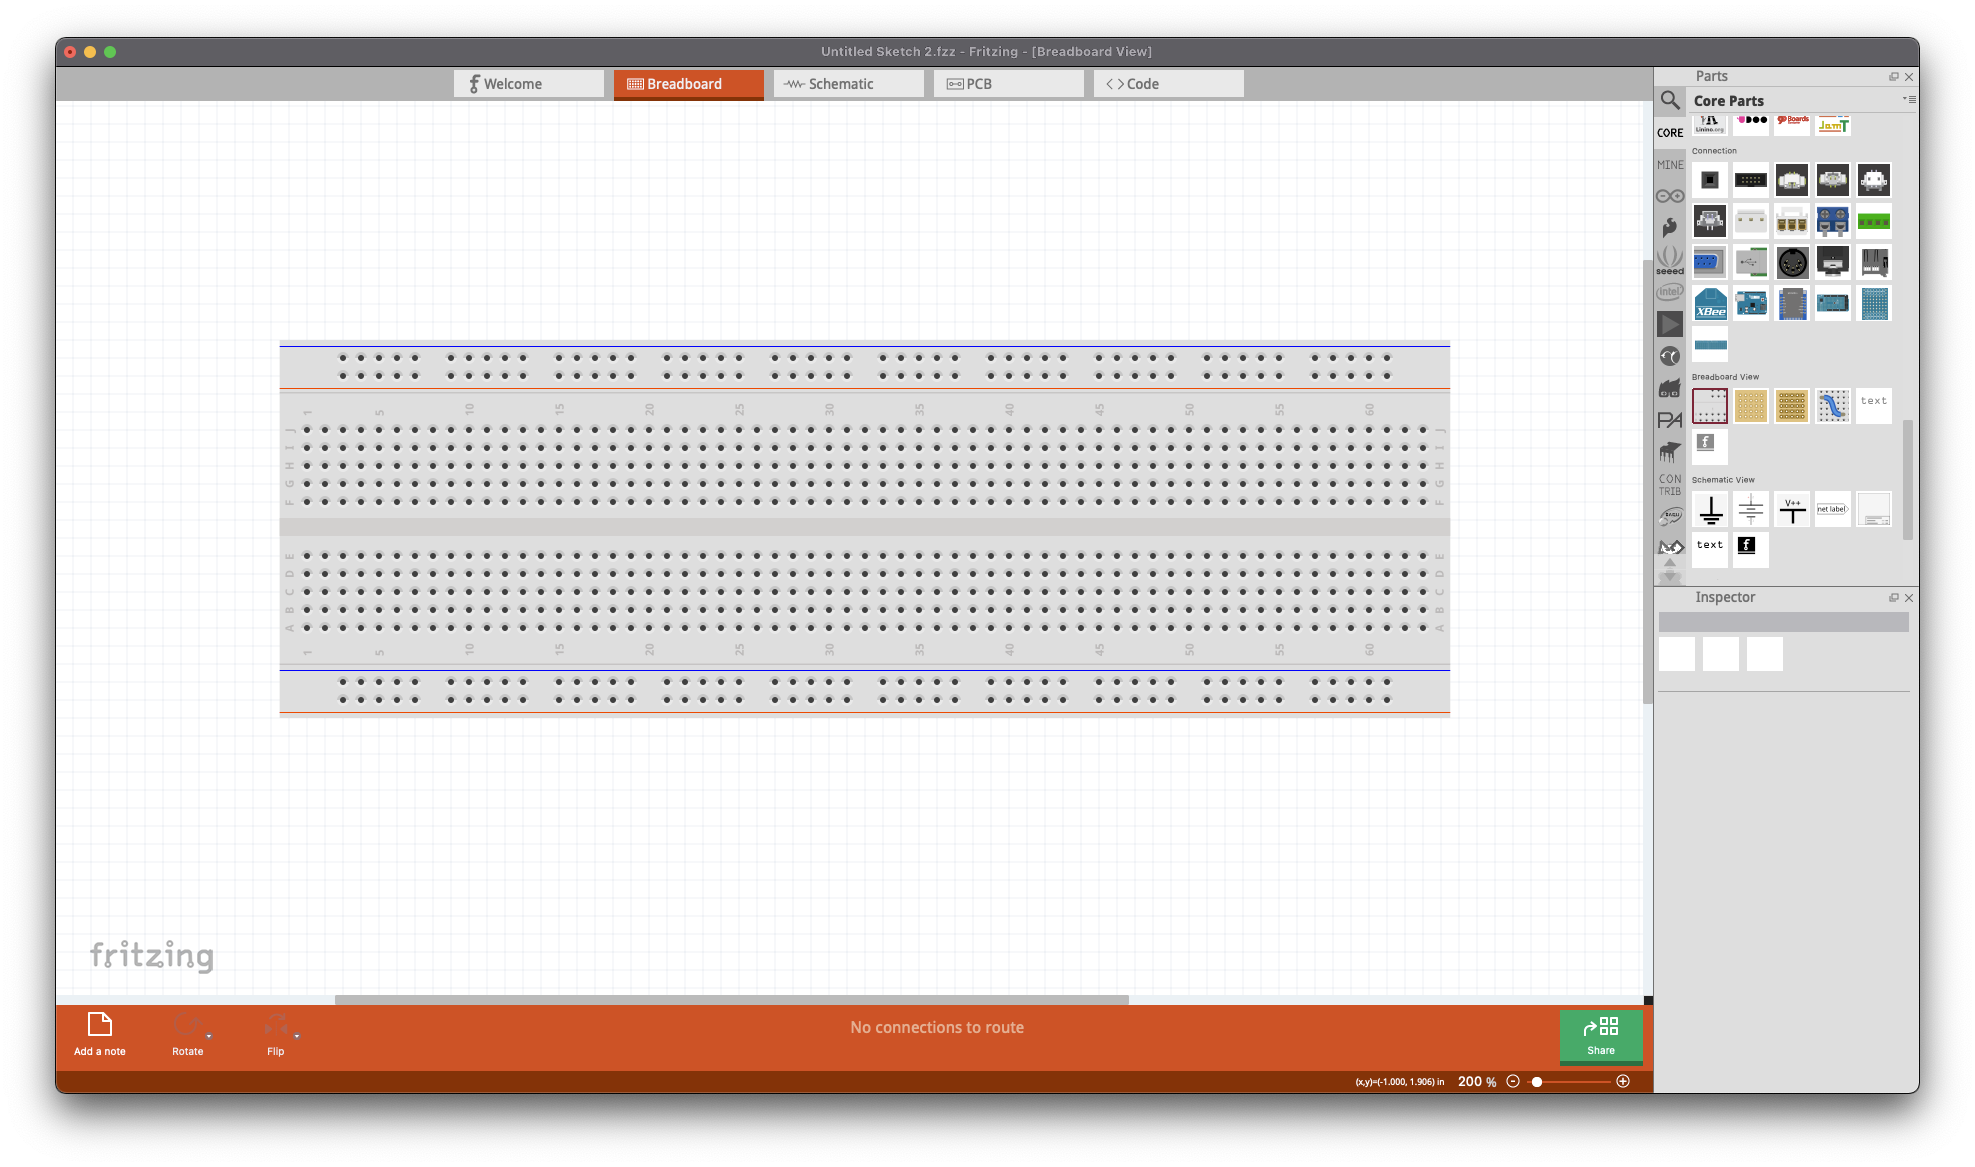
\includegraphics[scale=0.22]{introduction/1.png}    
\caption{محیط کار نرم‌افزار Fritzing}
\end{figure}
 
 
\section{اتصالات داخلی بردبورد}
در بالا و پایین برد بورد چهار نوار تغذیه وجود دارند که از هم مجزا هستند یعنی هیچ نواری
به نوار دیگر وصل نیست اما هر نوار در عرض کل برد بورد وصل است.
\begin{figure}[h!]
\centering
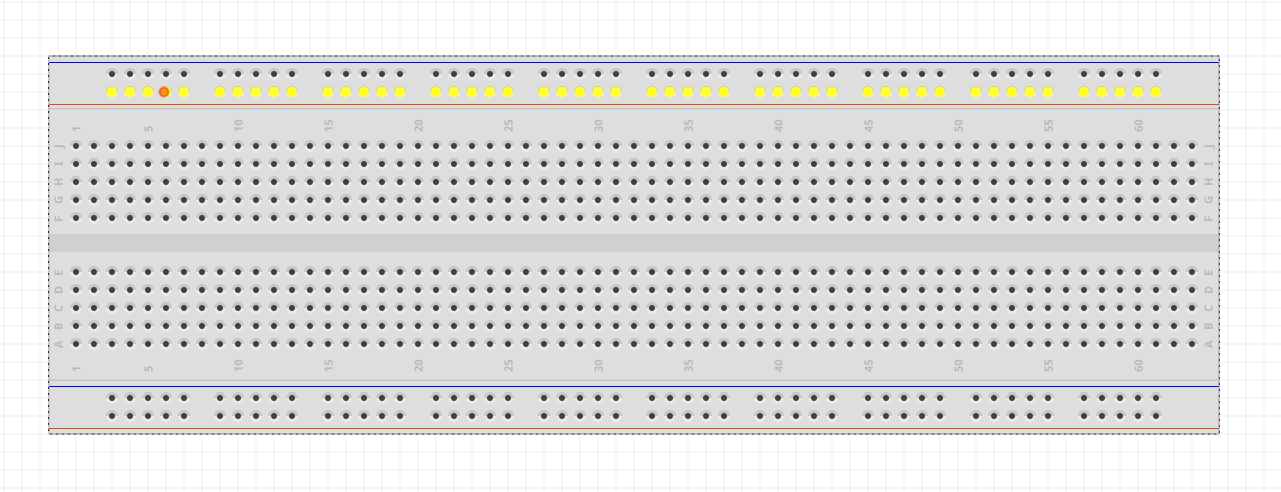
\includegraphics[scale=0.3]{introduction/3.png}    
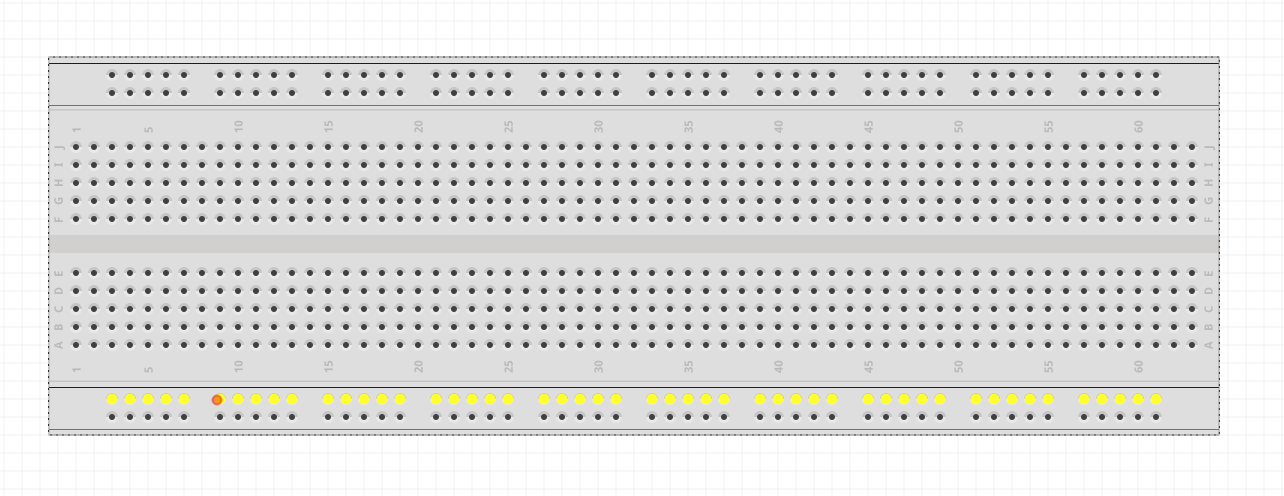
\includegraphics[scale=0.3]{introduction/4.png}    
\caption{دو تا از از نوارهای تغذیه بردبورد}
\end{figure}

در میانه‌ی برد بورد
ستون‌ها وجود دارند که هر ستون به اعضای خود وصل است.
اما ستون‌های بالا و پایین شکاف میانی به هم وصل نیستند.

\begin{figure}[h!]
\centering
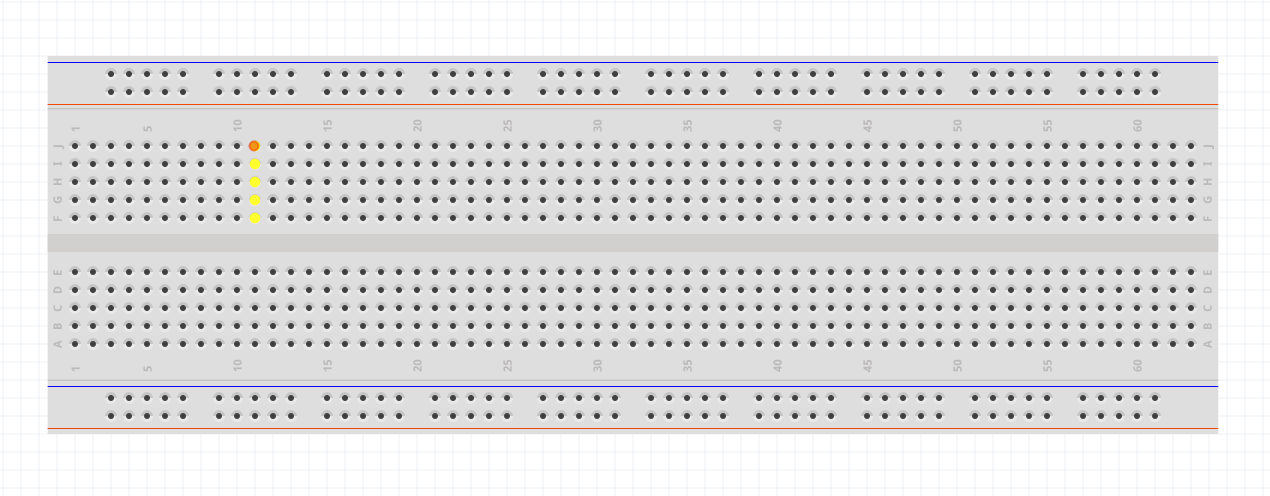
\includegraphics[scale=0.3]{introduction/2.png}    
\caption{یکی از ستون‌های اصلی}
\end{figure}

\section{
مدار LED
}
\subsection*{وسایل مورد نیاز}
\begin{enumerate}
    \item LED
    \item مقاومت 220 اهم
    \item منبع تغذیه 3 ولت
\end{enumerate}

\subsection*{تئوری آزمایش}
برای این آزمایش باید دقت کنیم پایه‌ّهای
LED
دارا جهت هستند و می‌بایست به مثبت و منفی بودن پایه‌ها دقت کرد.
برای تشخیص این امر به این نکته توجه می‌کنیم که داخل
LED
پایه‌ای که به تکه‌ی فلزی کوچک‌تر متصل است پایه‌ی مثبت است.
در صورتی که داخل LED
معلوم نبود به این نکته توجه داریم که معمولا پایه‌ی مثبت
LED
کمی بلند‌تر از پایه‌ی منفی است.

\begin{figure}[h!]
\centering
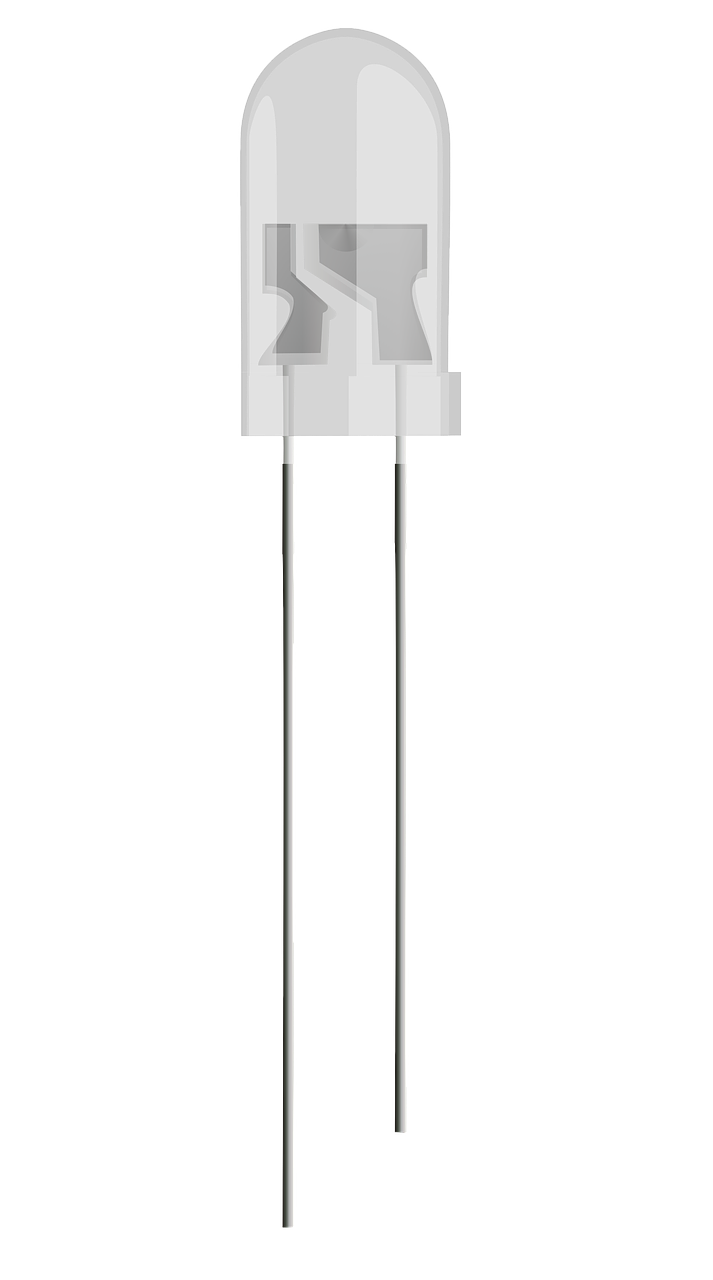
\includegraphics[scale=0.15]{introduction/led.png}    
\caption{یک LED معمولی}
\end{figure}

\subsection*{شرح آزمایش}
مطابق شکل مدار را به شکل صحیح بسته و به جهت پایه‌های
LED
توجه داریم.
همچنین برای تمیزی مدار باتری را به خطوط تغذیه بردبورد وصل می‌کنیم.
در ضمن اهمیتی ندارد مقاومت را در چه سمت
LED
قرار می‌دهیم زیرا در هر دو صورت معادله‌ی مدار یکسان است.


در انتها با قابلیت نرم‌افزار بررسی می‌کنیم تا اتصالات از ابتدای سر مثبت باتری تا جایی که
جریان به سر منفی می‌رسد برقرار باشد.

\begin{figure}[h]
\centering
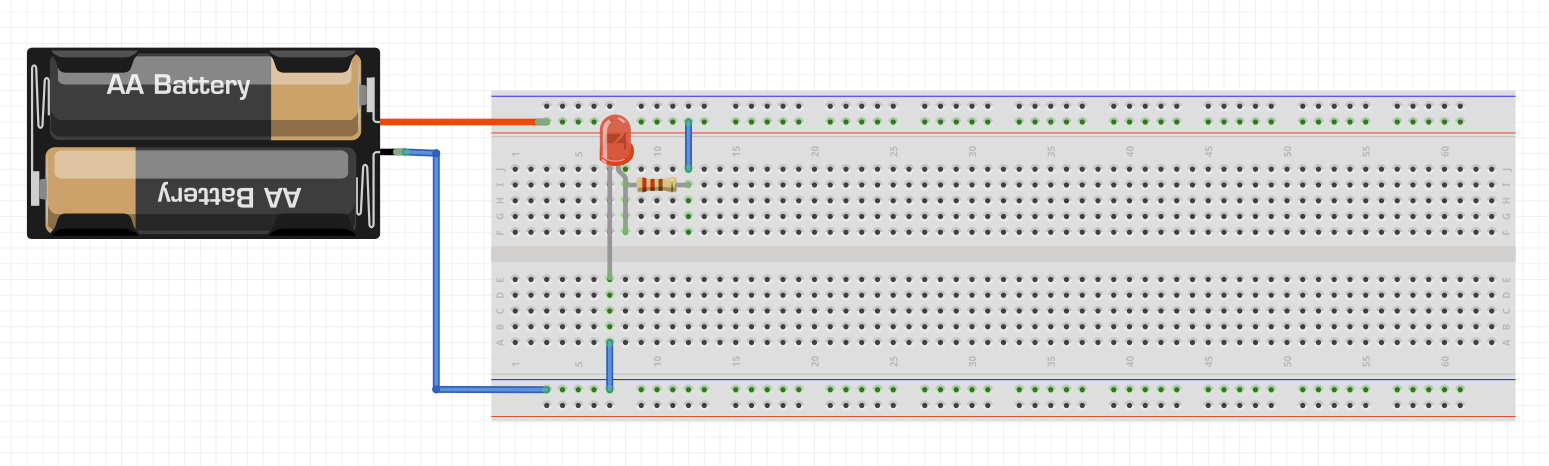
\includegraphics[scale=0.3]{introduction/5.png}    
\caption{مدار بخش ۲}
\end{figure}

\newpage
\section{نات نات نات نات نات نات}
\subsection*{وسایل مورد نیاز}
\begin{enumerate}
    \item LED
    \item 6 گیت نات
    \item منبع تغذیه 3 ولت
\end{enumerate}

\subsection*{تئوری آزمایش}
در نرم‌افزار به طور مستقیم قطعه‌ای با گیت نات وجود ندارد.
اما می‌دانیم با گیت
NOR
می‌توان گیت نات را ساخت.
برای این کار دو سر ورودی
NOR
را به هم وصل می‌کنیم.
با استفاده از دو آی‌سی
گیت
NOR
که هر کدام چهار گیت دارند، شش گیت نات مورد نیاز را خواهیم داشت.

\begin{figure}[h]
\centering
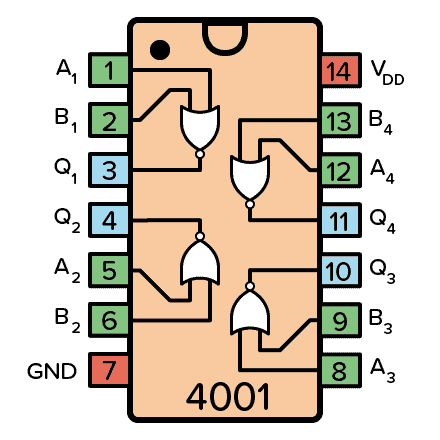
\includegraphics[scale=0.3]{introduction/not.png}    
\caption{مدار داخلی 4001}
\end{figure}

\subsection*{شرح آزمایش}
مطابق شکل ابتدا آی‌سی را روی شکاف بردبورد قرار داده و سپس تغذیه‌ی
آی‌سی‌ها را مطابق دیتاشیت‌شان
به آن‌ها وصل می‌کنیم.
معمولا پایه‌ی بالا سمت چپ VCC
و پایه‌ی پایین سمت راست
منفی یا زمین است.
دقت کنید که این بالا و پایین به شرطی است که نیم‌دایره‌ی فرورفته‌ی آی‌سی را در سمت چپ قرار دهیم و قطعه را نگاه کنیم.

حال که تغذیه‌ی آی‌سی‌ها وصل شد،
آن‌ها آماده‌ی کار هستند و آن‌ها را مطابق توضیحات بخش تئوری وصل می‌کنیم.


نکته‌ی مهم دیگر این که معمولا دیودهای نوری یا همان 
LED
برای ولتاژ حداکثر حدود
1.5 ولت طراحی شده‌اند.
که اینجا با اتصال باتری
3 
ولت بدون مقاومت ممکن است باعث سوختن LED
شویم.

همچنین بعضی از آی‌سی‌ها برای کار کردن به تغذیه‌ی بیشتر از 3 ولت
و در حدود 
5
ولت احتیاج دارند که اینجا فرض می‌کنیم هم LED و هم
آی‌سی با ولتاژ 3 ولت به درستی کار می‌کنند.


\begin{figure}[h]
\centering
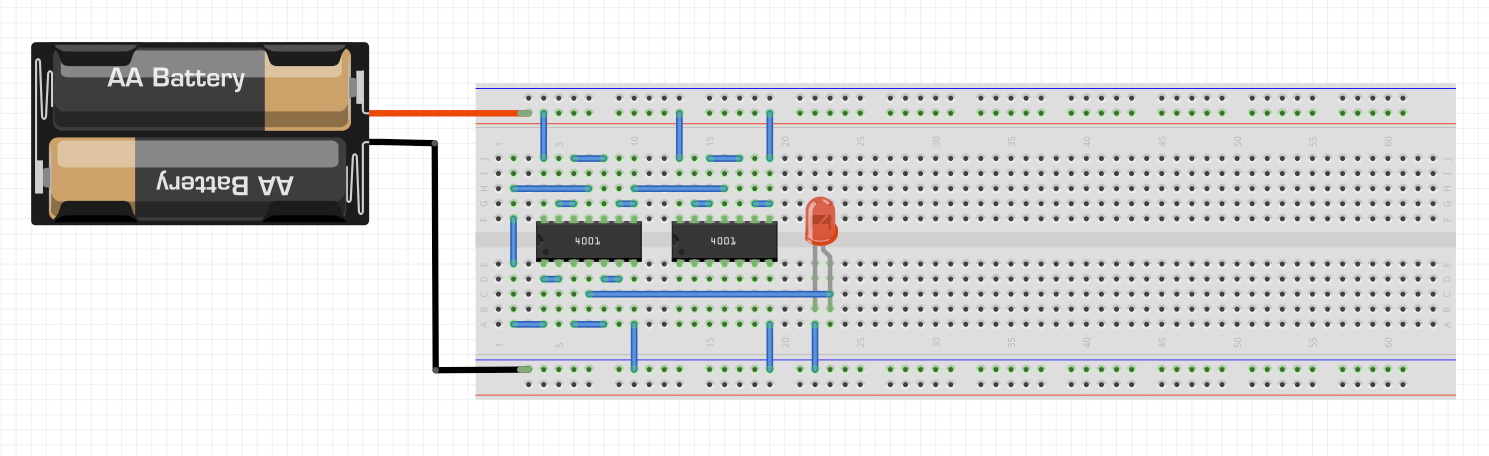
\includegraphics[scale=0.3]{introduction/6.png}    
\caption{مدار بخش 3}
\end{figure}
\chapter{
ساخت مدار با
Logisim
}
\section{جمع‌کننده کامل}
\subsection*{تئوری آزمایش}
Full Adder
یک مدار ترکیبی دیجیتال است که سه ورودی گرفته و دو خروجی می‌دهد.
یکی از این سه ورودی ره به عنوان کری ورودی می‌شناسیم و دو تای دیگر متغییرهایی هستند که قرار است جمع شوند.
خروجی این مدار نیز یکی بیت جمع و دیگر بیت کری خروجی است.

\begin{figure}[h]
\centering
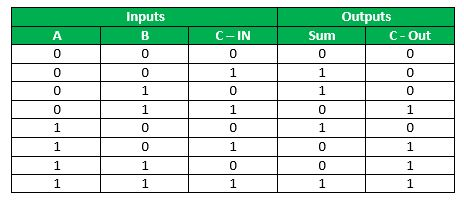
\includegraphics[scale=1]{Experimental Methods/table.jpg}
\caption{جدول صحت
یک جمع کننده کامل
}
\end{figure}

مطابق این جدول برای بیت‌های خروجی یک مدار بدست می‌آید که آن را در نرم‌افزار رسم کرده و شبیه‌سازی می‌کنیم.

\subsection{شرح آزمایش}
\begin{figure}[h]
\centering
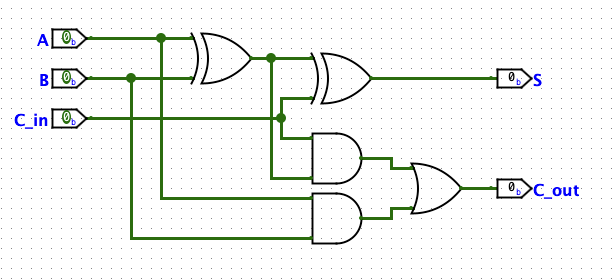
\includegraphics[scale=0.6]{Experimental Methods/1.png}
\caption{
مدار جمع‌کننده کامل در نرم‌افزار
Logisim
}
\end{figure}

ورودی‌ها و خروجی‌ها را به تعداد مناسب قرار داده و برای آن‌ها لیبل مناسب می‌زنیم.

حال گیت‌ها را قرار داده و اتصالات را برقرار می‌کنیم.

در نهایت با استفاده از ابزار
«دست»
که از منوی بالای صفحه قابل انتخاب است ورودی‌های مدار را تغییر می‌دهیم و تاثیر آن را در خروجی‌ها می‌بینیم.


\section{
جمع‌کننده/تفریق‌کننده
4 بیتی
}
برای کم کردن
B
از
A
کافی است هر دو عدد را در مکمل دو ببریم و سپس با جمع کننده‌ی عادی آن‌ها را جمع بزنیم.
حاصل نیز در مکمل دو خواهد بود.

همچنین می‌دانیم برای پیدا کردن مکمل دوی یک عدد باید بیت‌های آن را معکوس کرده سپس عدد نهایی را با یک جمع کنیم.
برای معکوس کردن بیت‌ها کافی است آن‌ها را با ورودی‌ای که اگر یک شود این اتفاق بیفتد
XOR کنیم.
که اگر این ورودی کنترلی یک باشد خروجی معکوس بیت‌ها و در غیر این صورت خود آن‌ها خواهد بود.

حالا این ورودی‌های معکوس شده‌ی مشروط را با هم جمع می‌کنیم. آن یکی هم که باید جمع می‌کردیم را در کری ورودی جمع‌کننده‌ی ابتدایی قرار می‌دهیم. نتیجه‌ی نهایی در شکل آمده است.

\begin{figure}[h]
\centering
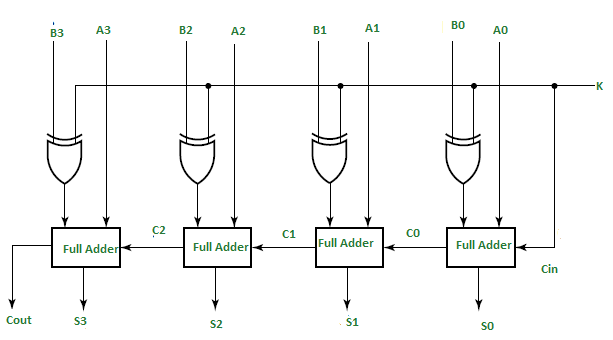
\includegraphics[scale=1]{Experimental Methods/2.png}
\caption{
شماتیک مدار جمع‌کننده/تفریق‌کننده کنترلی
}
\end{figure}

\subsection*{شرح آزمایش}
مطابق شکل نشان‌داده شده و مطابق مدار جمع کننده‌ی کامل که در بخش قبل بستیم مدار نهایی را می‌بندیم.

در انتها می‌توانیم کمی با آن بازی کنیم و آن را برای حالات مختلف تست کنیم.

\begin{figure}[h]
\centering
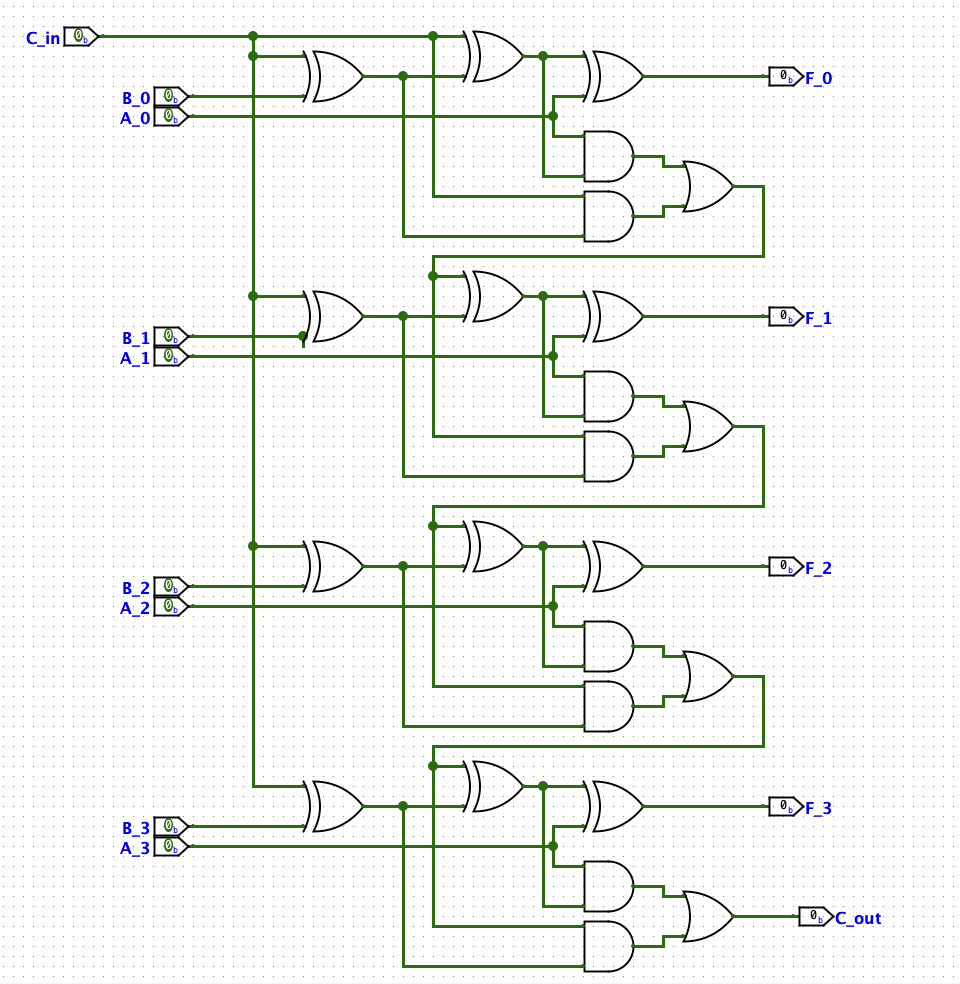
\includegraphics[scale=0.3]{Experimental Methods/3.png}
\caption{
مدار نهایی
}
\end{figure}
\chapter{
ساخت مدار با
Proteus
}
\section{جمع کننده‌ی Carry-Look-Ahead}
\subsection*{مقدمه و تئوری آزمایش}
برای ساخت جمع‌کننده‌هایی با تعداد بیت‌بالا معمول است که جمع‌کننده‌های کوچک را پشت سر هم می‌بندند.
این کار از جهاتی بسیار مفید است. چرا که به تمیزتر شدن مدار و قطعه‌قطعه یا ماژولار شدن آن کمک می‌کند.
اما مشکلی که این روش دارد این است که هر جمع کننده برای رسیدن به جواب نهایی باید بیت کری ورودی خود را بداند و این عدم آگاهی زنجیروار تا اولین جمع‌کنند می‌رسد به طوری که جمع‌کننده‌ی بیت آخر باید به تعداد تاخیر همه‌ی جمع‌کننده‌های قبلی خود صبر کند تا جواب قطعی درست بدهد.

برای حل این مشکل از قطعه‌ای به نام
\lr{Carry Look-ahead Generator}
استفاده می‌شود که به طور خلاصه این زمان تاخیر را کاهش می‌دهد و کری‌ها را با سرعت بالاتری محاسبه می‌کند و در اختیار جمع‌کننده‌های دیگر می‌گذارد. و در واقع این وابستگی پشت هم قطعات و جمع شدن تاخیر آن‌ها را از بین می‌برد.

\begin{figure}[h]
\centering
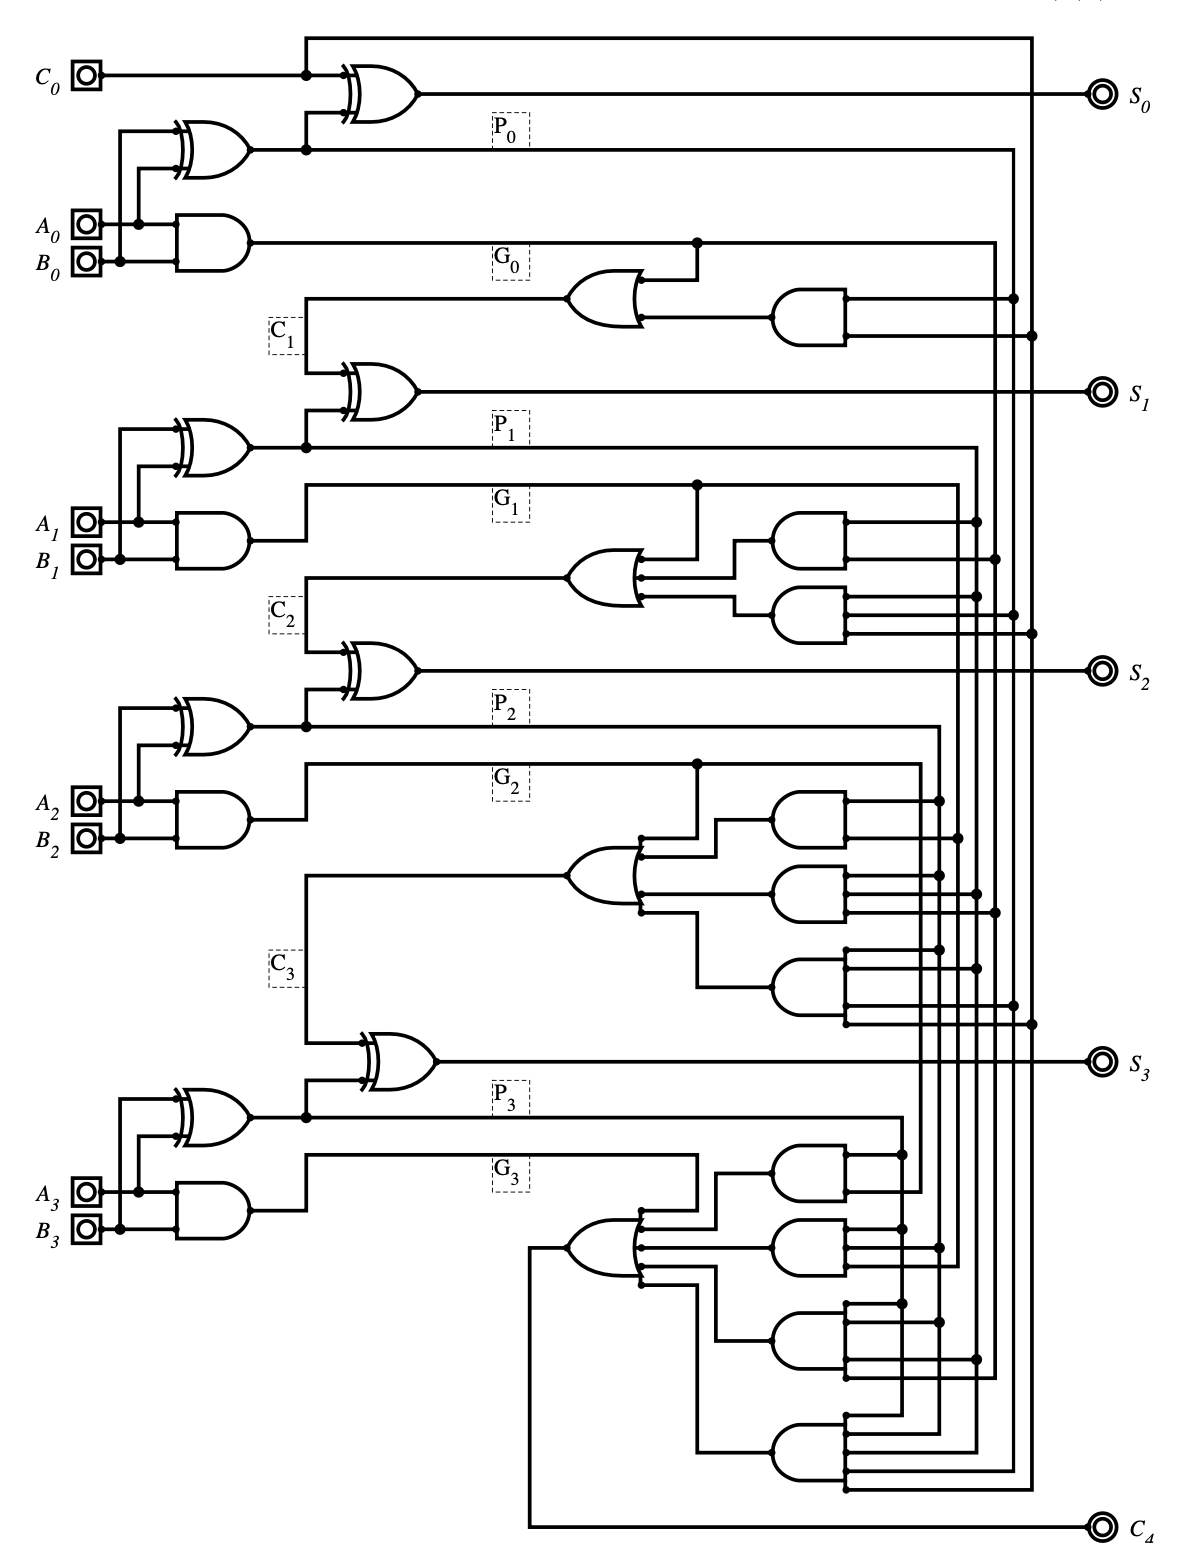
\includegraphics[scale=0.7]{Results/3.png}
\caption{
مدار داخلی یک
جمع کننده 4 بیت با
\lr{Carry Look-ahead Generator}
باز
}
\end{figure}

\subsection*{شرح آزمایش}
\begin{figure}[h]
\centering
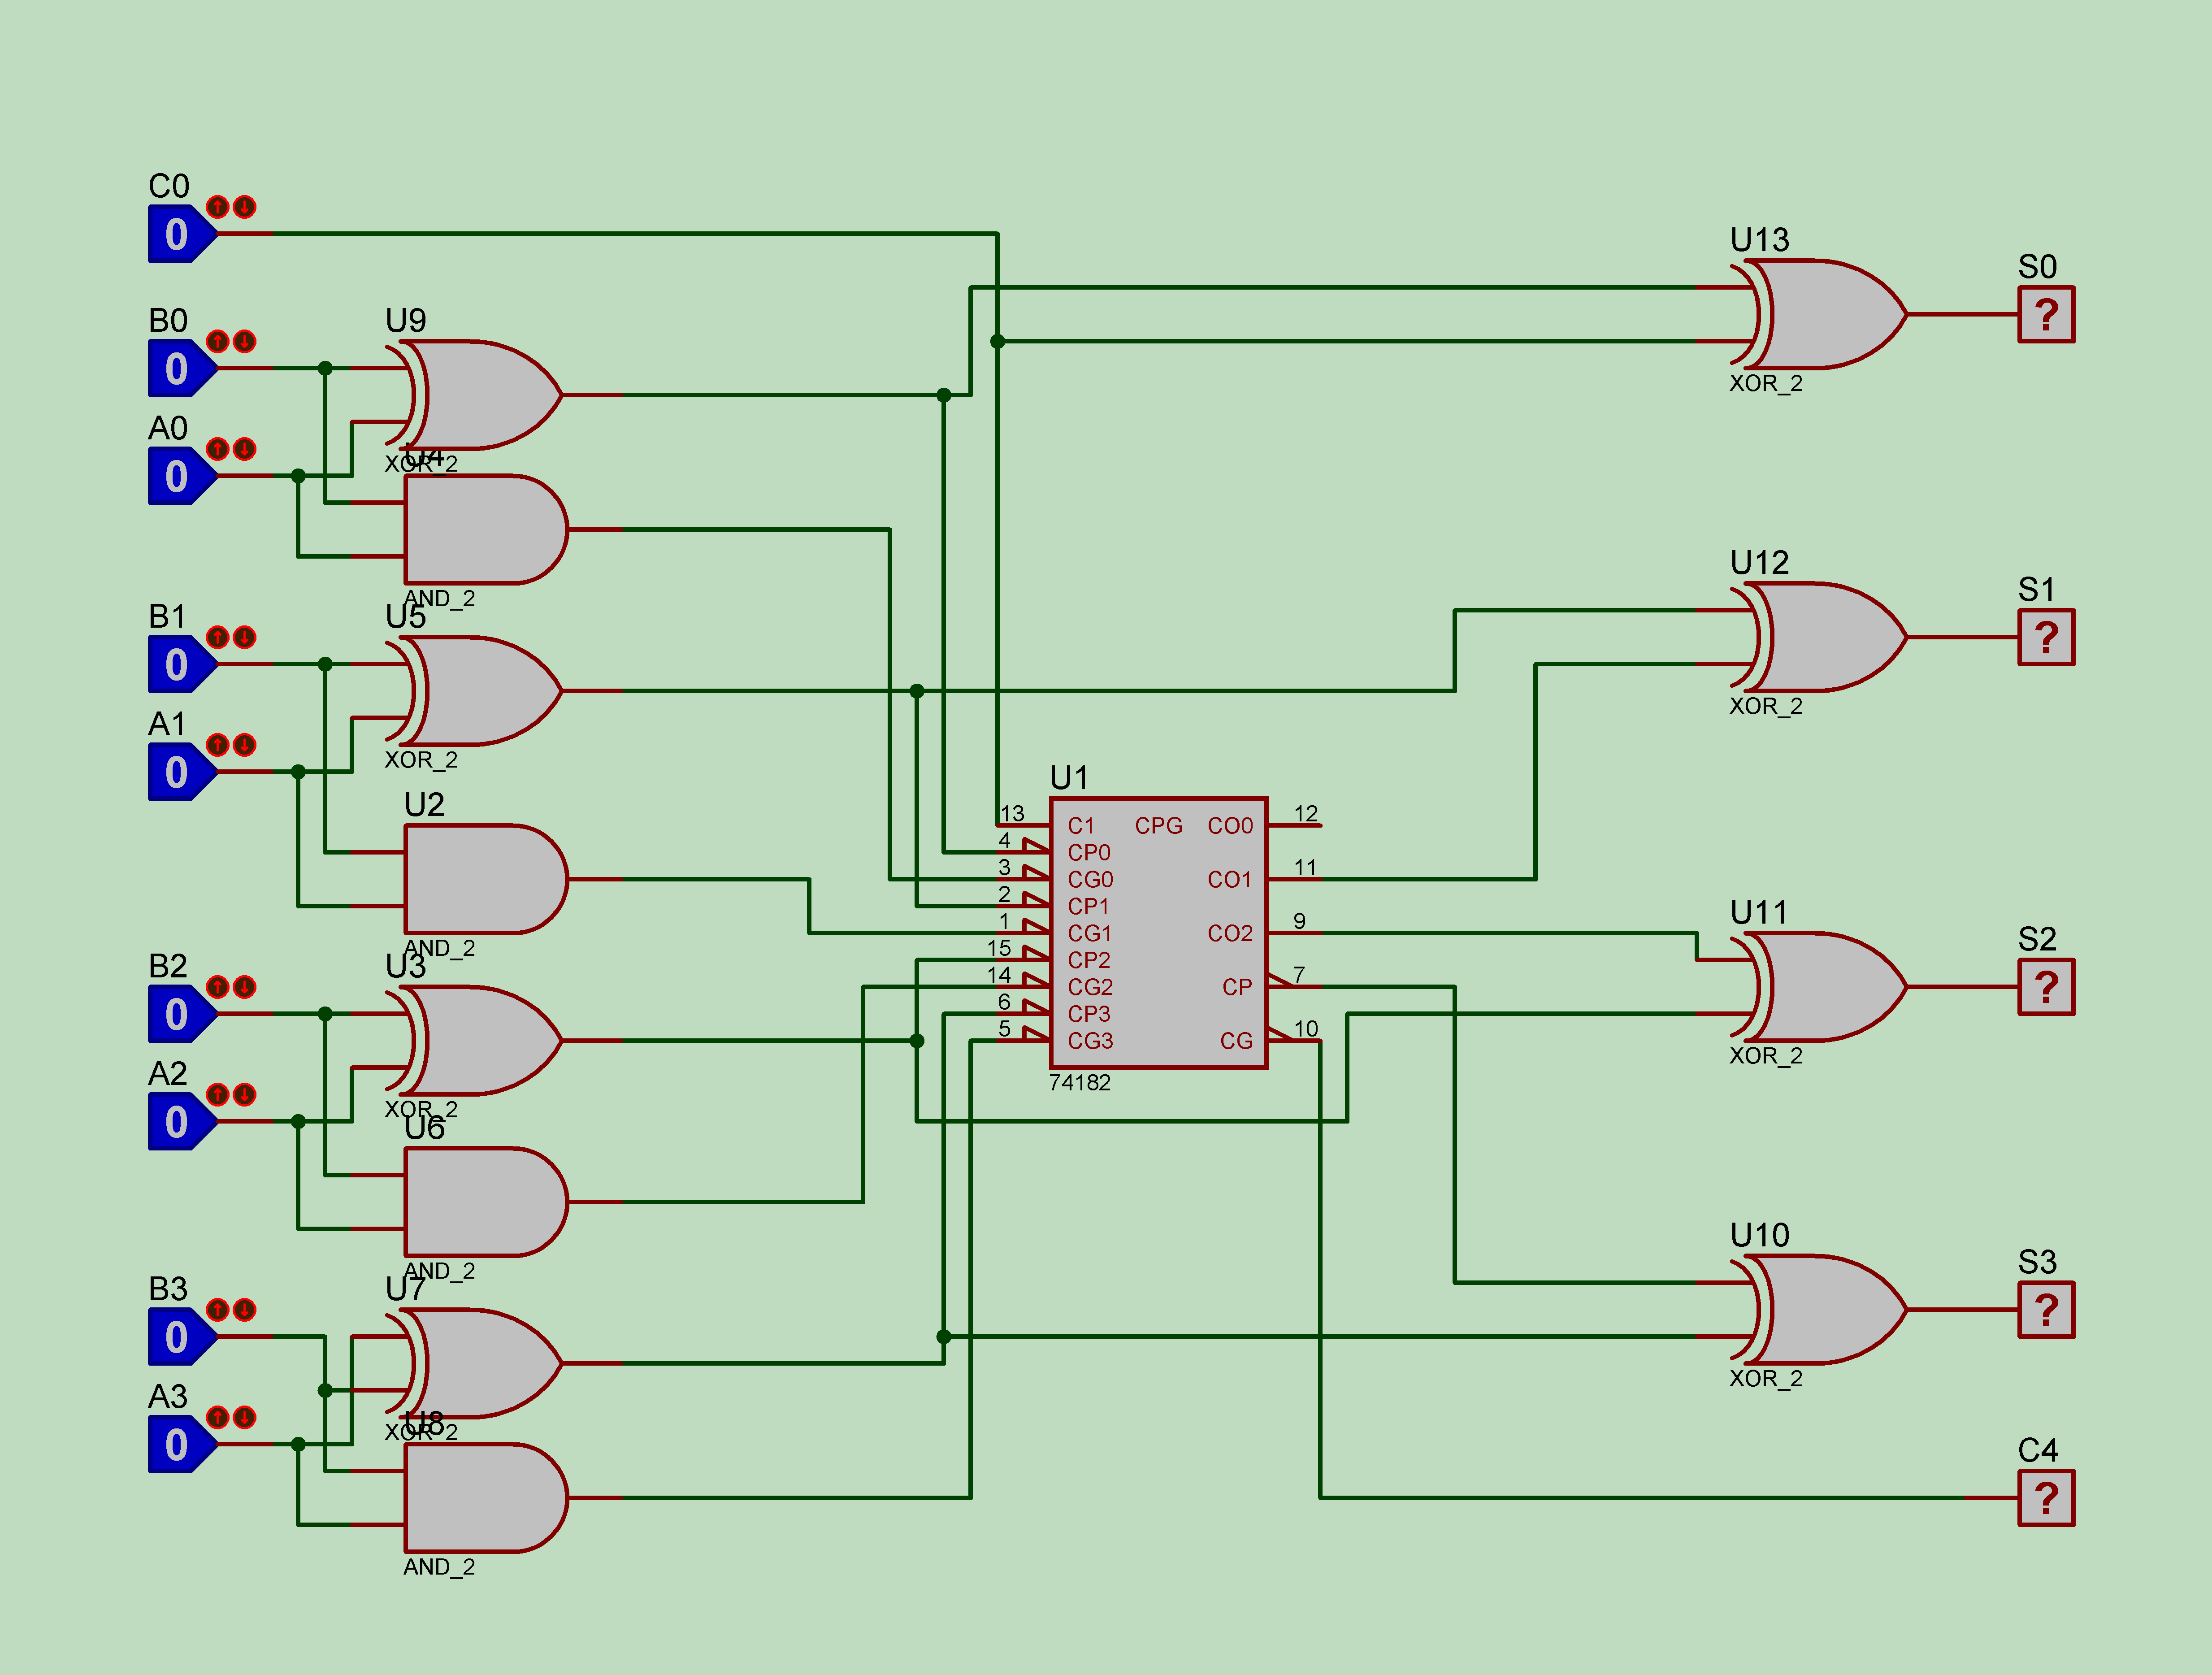
\includegraphics[scale=0.09]{Results/FastAdder.png}
\caption{
جمع کننده‌ی 4 بیتی سریع
}
\end{figure}

مطابق شکل قطعه‌ی 
\lr{Carry Look-ahead Generator}
را از کتابخانه‌ی نرم‌افزار
Proteus
پیدا کرده و قرار می‌دهیم سپس مطابق تئوری گیت‌ها و ورودی‌ها و خروجی‌ها را وصل می‌کنیم و برای آن‌ها نام می‌گذاریم.


\chapter{نتیجه و بحث}
در اولین جلسه از آزمایشگاه مدارهای منطقی با کار با سه نرم‌افزار مهم آشنا شدیم.

\begin{figure}[h]
\centering

\includegraphics[scale=0.4]{conclusion/fritzing.png}
\caption{
لوگوی نرم‌افزار
Fritzing}
\end{figure}

نرم‌افزار اول
Fritzing
بود که اوپن‌سورس است ولی قابلیت‌های چندانی از جمله شبیه‌سازی ندارد و تنها برای طراحی مدارات و قطعات است. البته از مزیت‌های این برنامه نزدیک به واقعیت بودن قطعات است و این امر برای طراحی بسیار مناسب است.

\begin{figure}[h]
\centering
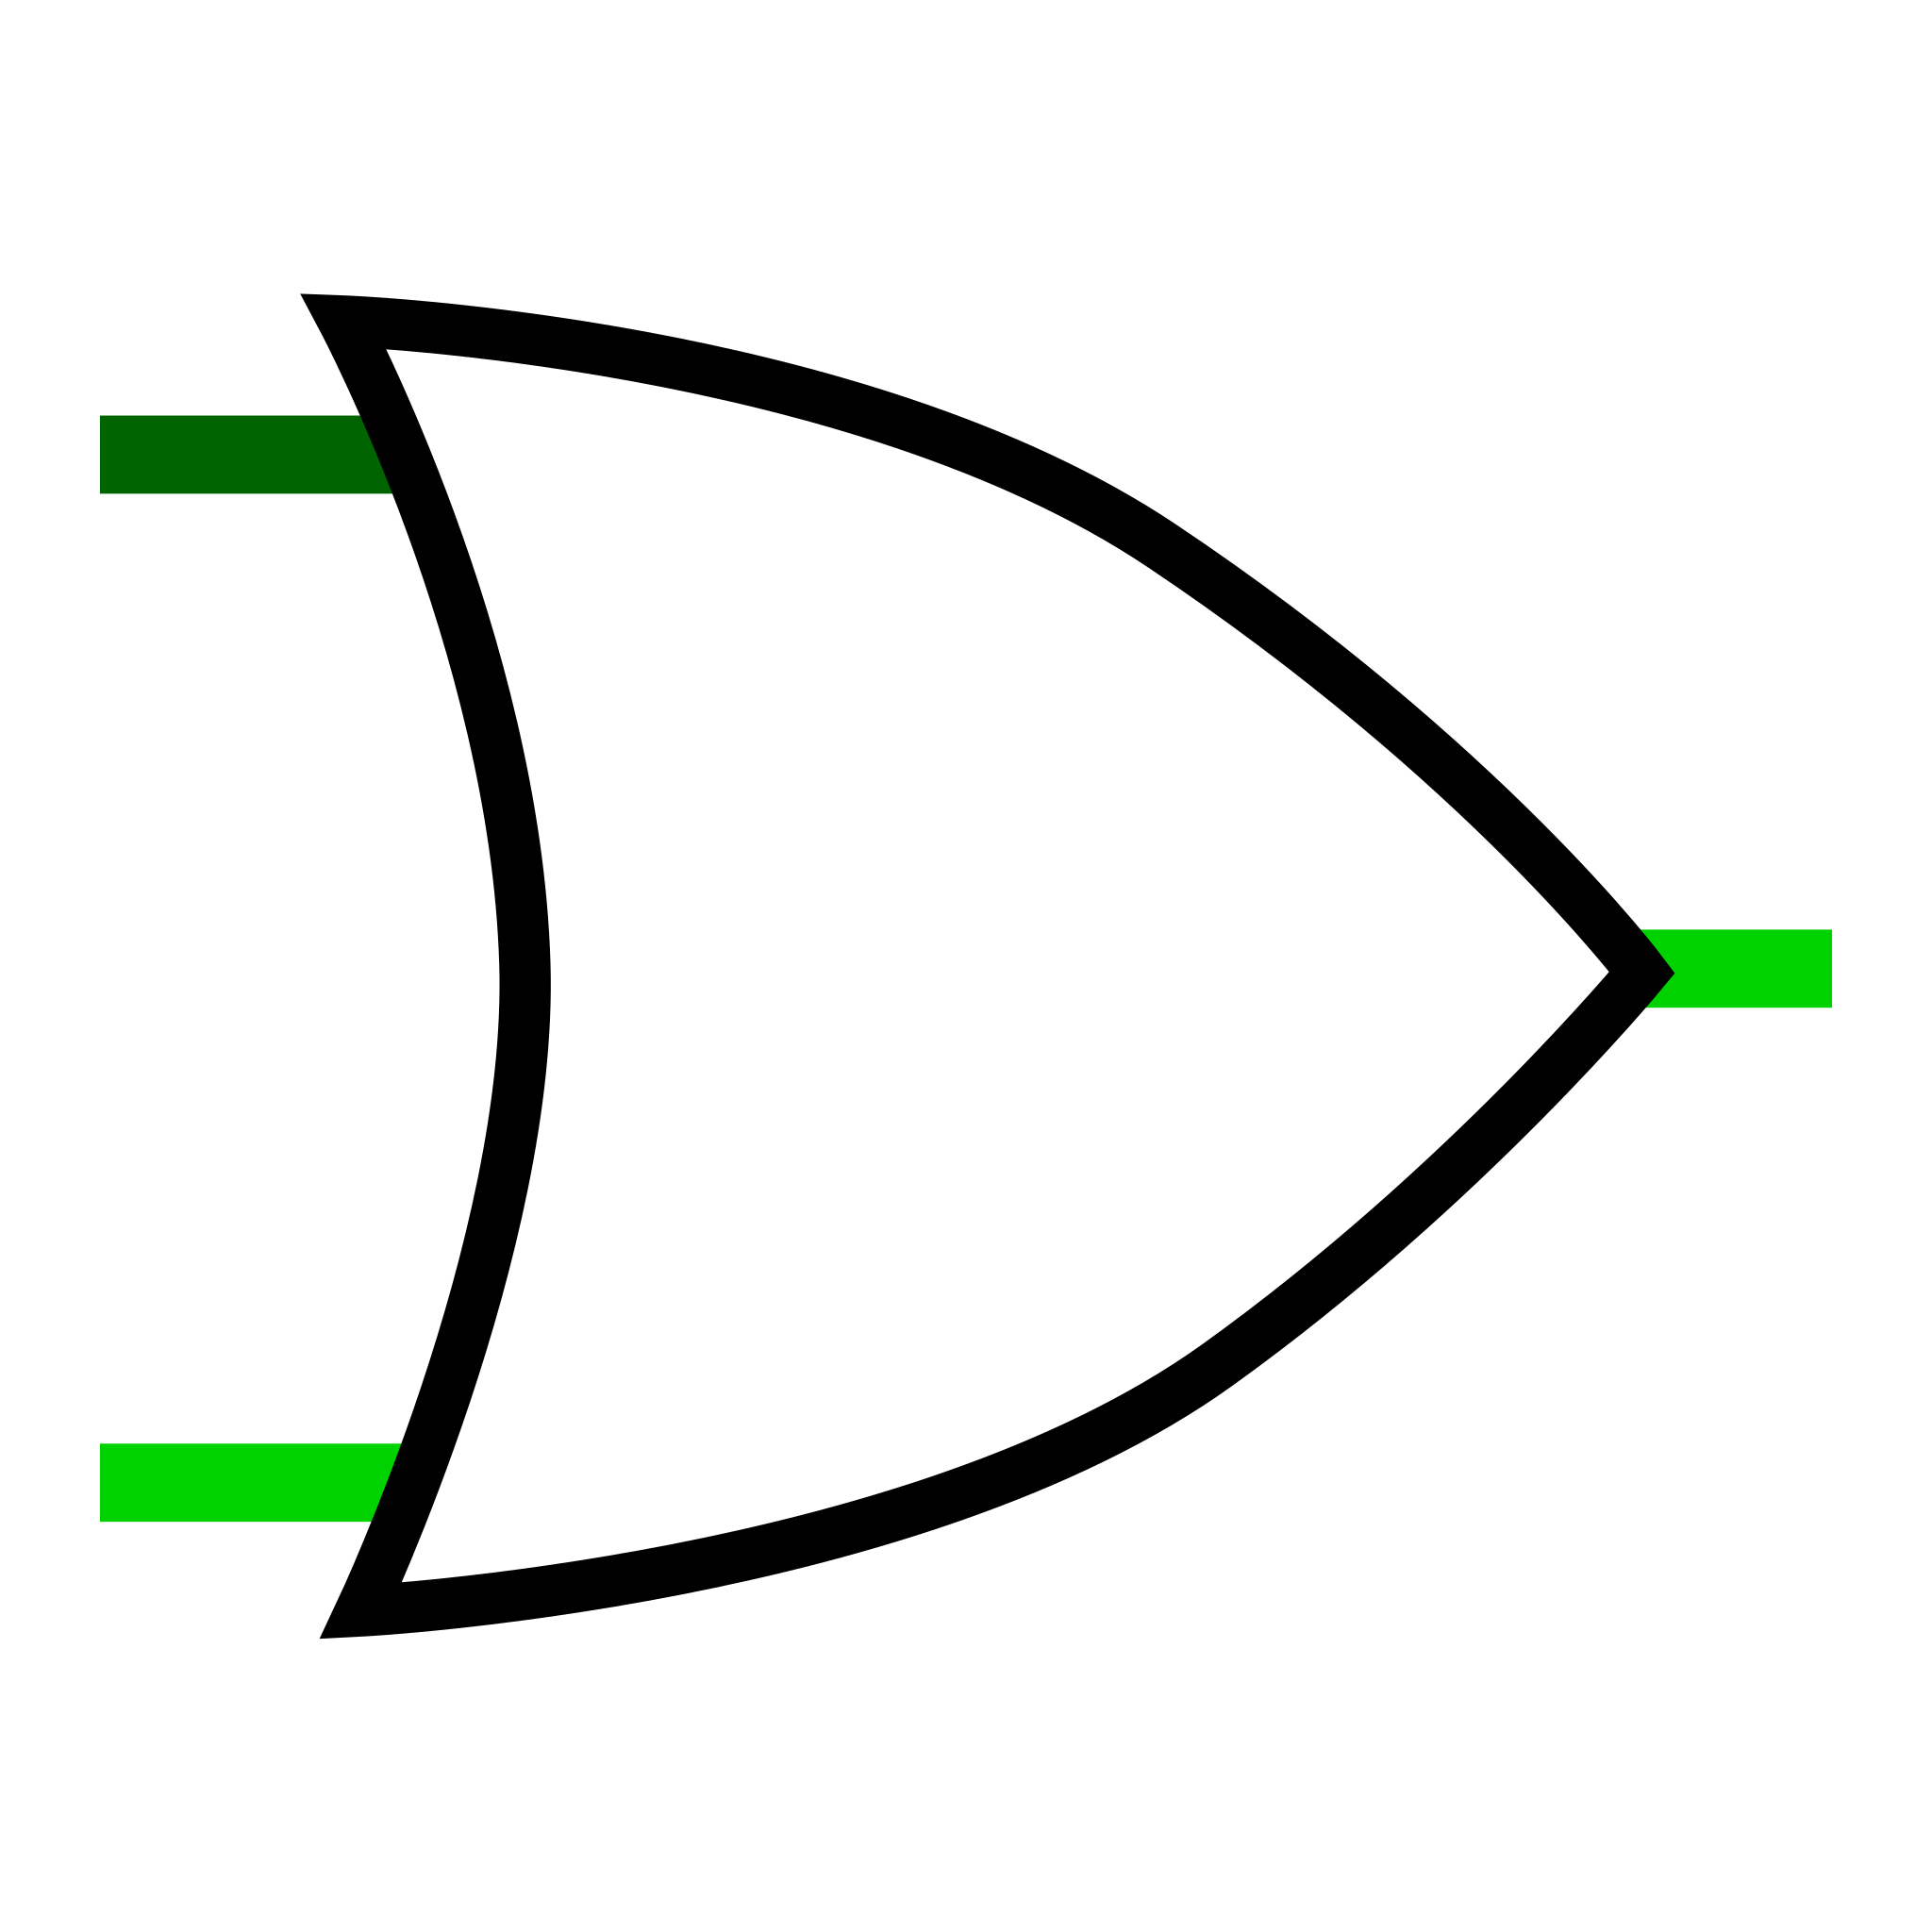
\includegraphics[scale=0.035]{conclusion/logisim.png}
\caption{
لوگوی نرم‌افزار
Logisim}
\end{figure}

نرم افزار دومی که با آن کار کردیم
Logisim
بود که این هم اوپن سورس است و ظاهر بسیار ساده‌ای دارد اما این یکی بر خلاف قبلی امکان شبیه‌سازی مدارها را به صورت در لحظه دارد به طوری که در حین اجرا نیز می‌توان ورودی‌ها را تغییر داد و نتیجه را درجا مشاهده کرد.
اما محدودیت این نرم‌افزار در کم بودن تنوع قطعات و ساده بودنش است به طوری که تنها گیت‌ها و برخی قطعات محدود را می‌توان در آن استفاده کرد.

\begin{figure}[h!]
\centering

\includegraphics[scale=0.3]{conclusion/proteus.png}
\caption{
لوگوی نرم‌افزار
Proteus}
\end{figure}

در انتها به نرم‌افزار
معروف
پولی فقط ویندوزی
Proteus
رسیدیم.
این نرم‌افزار ظاهر شلوغ و اعصاب خردکنی دارد اما در عوض بسیار کامل بوده و امکانات بسیار زیادی داردو همچنین تنوع قطعات آن بسیار فراوان است و گاه از زیاد بودن تنوع و مدل‌های یک قطعه اعصاب آزمایشگر را خرد می‌کند. 
اما در نهایت این تنوع و امکانات زیاد و امکان شبیه‌سازی بسیار خود آن باعث شده برای اکثر مدارها فراتر از نیاز آزمایشگر باشد.
\bibliographystyle{unsrtnat}
%\bibliography{bibs/sample}

\end{document}